\underline{Exercise 9.2}
\begin{enumerate}
% Question 1
\item[1.]
\begin{enumerate}
\item[(c)] $y = 3x^{2} + 3$
\[\frac{dy}{dx} = 6x = 0 \;\Rightarrow\; x^{*} = 0\]
In the immediate neighborhood of $0$, $dy/dx < 0$ for $x < 0$ and $dy/dx > 0$ for $x > 0$. The slope changes sign from negative to positive, so the function is decreasing to the left of $0$ and increasing to the right: $f(0) = 3$ is a relative minimum. The second derivative confirms this: $d^{2}y/dx^{2} = 6 > 0$.
\begin{center}
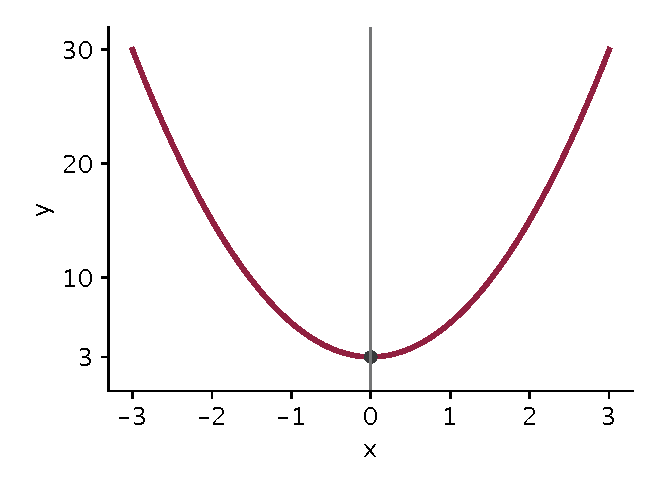
\includegraphics[width=0.42\textwidth,alt={The upward-opening parabola y equals 3 x squared plus 3, symmetric about the vertical axis, with a dot at its lowest point (0, 3)}]{../../latex/fig/quad-min.pdf}
\end{center}
\end{enumerate}

% Question 2
\item[2.]
\begin{enumerate}
\item[(a)] $y = x^{3} - 3x + 5$
\[\frac{dy}{dx} = 3x^{2} - 3 = 0 \;\Rightarrow\; x^{*} = \pm 1\]
The derivative $3(x^{2} - 1)$ is negative on the immediate left of $1$ (for example at $0.9$) and positive on the immediate right (at $1.1$), so there is a relative minimum at $x = 1$. It is positive on the immediate left of $-1$ and negative on the right, so there would be a relative maximum at $x = -1$. But the domain is $[0, \infty)$, so $-1$ is not admissible. The only stationary value is the relative minimum $f(1) = 3$. The second-derivative test gives the same answer: $d^{2}y/dx^{2} = 6x$, which is $6 > 0$ at $x = 1$.
\begin{center}
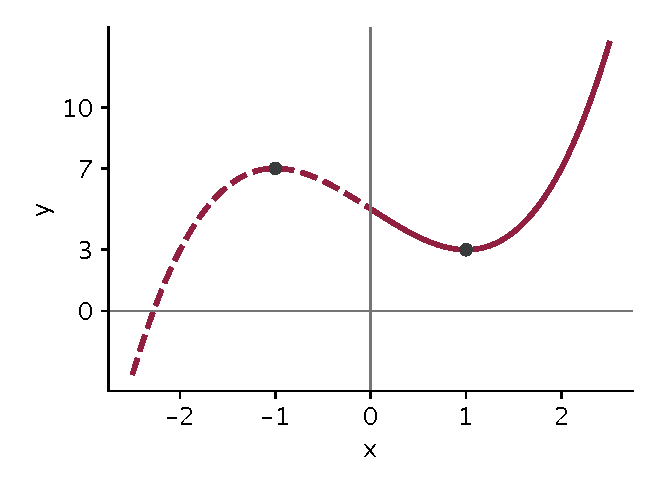
\includegraphics[width=0.42\textwidth,alt={The curve y equals x cubed minus 3 x plus 5, drawn solid for x at least 0 and dashed for negative x. Dots mark the local minimum at (1, 3) on the solid part and the local maximum at (negative 1, 7) on the dashed part}]{../../latex/fig/cubic-hw.pdf}
\end{center}
\end{enumerate}

% Question 3
\item[3.] $f(x) = x + 1/x$
\[f'(x) = 1 - \frac{1}{x^{2}} = 0 \;\Rightarrow\; x^{*} = \pm 1\]
The derivative, $(x^{2} - 1)/x^{2}$, is negative on the immediate left of $1$ and positive on the immediate right, so $f(1) = 2$ is a relative minimum. It is positive on the immediate left of $-1$ and negative on the right, so $f(-1) = -2$ is a relative maximum.

The relative maximum, $-2$, is lower than the relative minimum, $2$. This is not a contradiction: these are \textit{relative} extrema, each compared only with nearby points on its own branch of the graph. The function is not defined at $x = 0$, and the two branches never meet.
\begin{center}
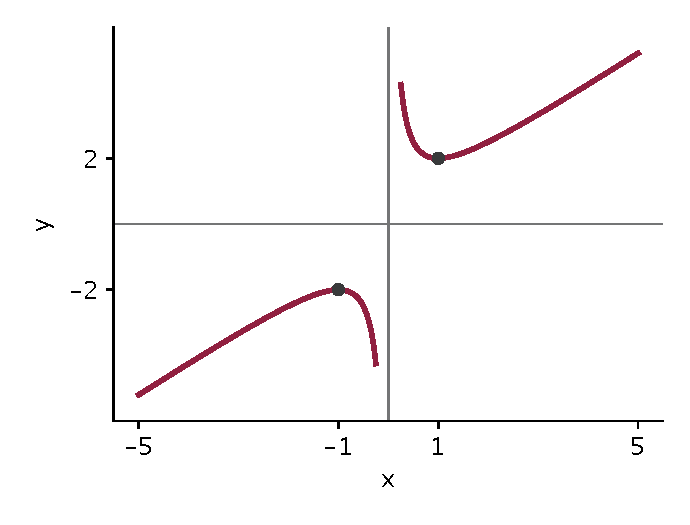
\includegraphics[width=0.45\textwidth,alt={The two branches of y equals x plus 1 over x. The right branch, for positive x, has a dot at its lowest point (1, 2); the left branch, for negative x, has a dot at its highest point (negative 1, negative 2), which lies below the minimum of the right branch}]{../../latex/fig/x-plus-recip.pdf}
\end{center}

% Question 4
\item[4.] $T = \phi(x)$
\begin{enumerate}
\item[(a)] $M = \phi'(x)$ and $A = \phi(x)/x$.
\item[(b)] At an extremum of $A$,
\[A' = \frac{\phi'(x)\, x - \phi(x)}{x^{2}} = 0 \;\Rightarrow\; \phi'(x^{*}) = \frac{\phi(x^{*})}{x^{*}}\]
that is, $M = A$.
\item[(c)] The marginal curve must cross the average curve at the point where the average curve reaches its extremum (its lowest point for a U-shaped average cost curve).
\item[(d)] The elasticity of $T$ is
\[\varepsilon = \frac{\phi'(x)\, x}{\phi(x)} = \frac{M}{A}\]
When $M = A$, the elasticity equals $1$.
\end{enumerate}

\end{enumerate}
